%\section[Overview]{Overview
\chapter[Overview]{Overview
\footnote{
  $CVS~revision~ $Id: overview.tex,v 1.10 2003/12/13 06:23:38 gen Exp $ $
}
\footnote{Authors: Dr. B.B.Wojtsekhowski \email{bogdanw@jlab.org}}
}
\label{chap:hrs_det}

\section{Overview of the Detector Package}

The detector packages of the two spectrometers are designed 
to perform various functions 
in the characterization of charged particles passing through the spectrometer. 
These include: providing a trigger to activate the data-acquisition 
electronics, collecting tracking information (position and direction), 
precise timing for time-of-flight measurements and coincidence determination, 
and identification of the scattered particles. 
The timing information is provided from scintillators, as well as the
main trigger. The particle identification is obtained from a 
variety of \Cherenkov{}  type detectors (aerogel and gas) and 
lead-glass shower counters. 
A pair of VDCs provides tracking information.
The main part of the detector package in the two spectrometers 
(trigger scintillators and VDCs) is identical; 
the arrangement of particle-identification detectors differs slightly.
The HRS-L can be equipped with a focal-plane polarimeter to determine 
the polarization of detected protons.
The focal-plane-polarimeter operates with proton momenta up 
to 3 GeV/$c$ with figure-of-merit of 0.03.
The side view of the detector stacks are shown in Fig.~\ref{fig:side-view}.
%
\begin{figure}[p]
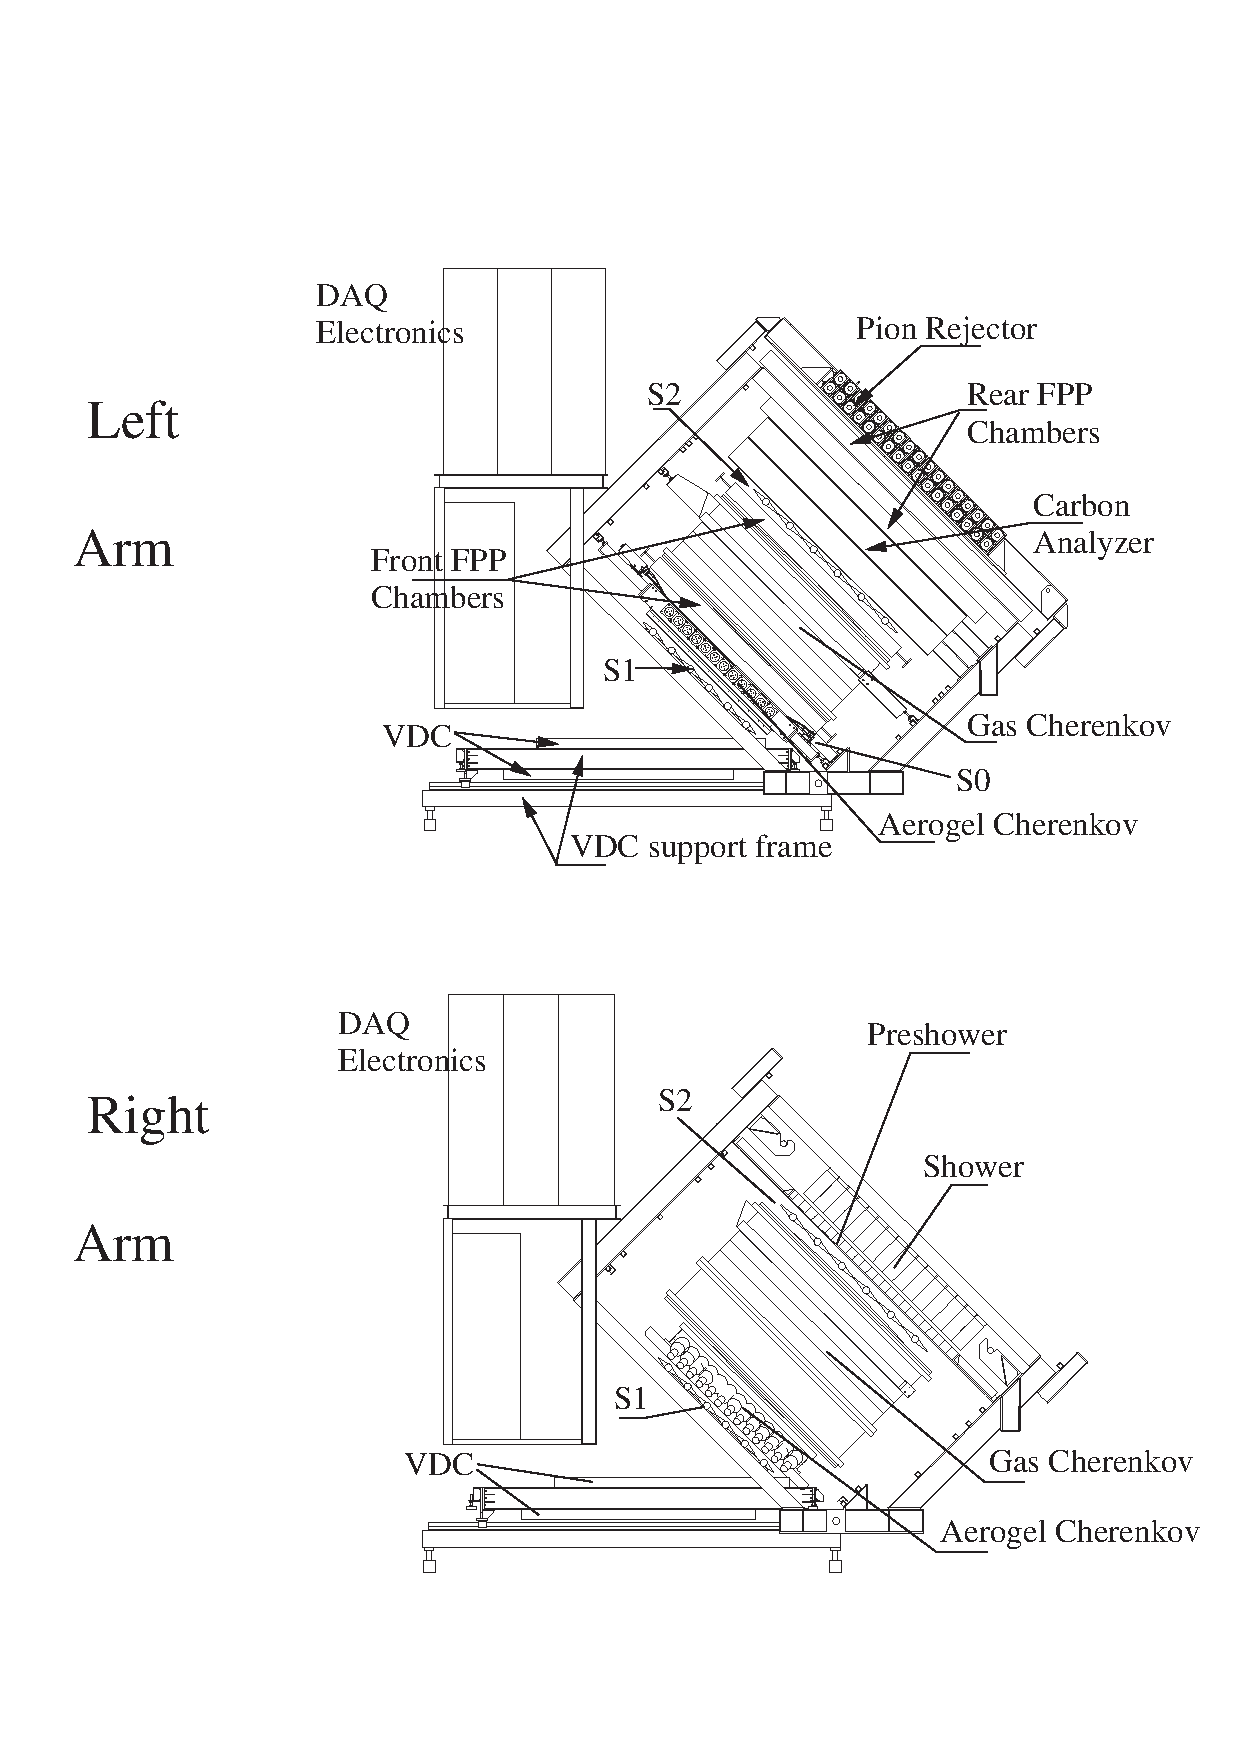
\includegraphics[angle=0,height=0.7\textheight]{hrs_det_sideview}
\caption[The side view of the detector stacks]
{The side view of the detector stacks.}
\label{fig:side-view}
\end{figure}
%

The optics of the HRS spectrometers, results in a narrow distribution of 
particle trajectories in the transverse direction, leading 
to an aspect ratio of the beam envelope of about 20:1 at 
the beginning of the detector package and 4:1 at the end.

The detector package and all data-acquisition (DAQ) electronics are located 
inside a Shield Hut (SH) to protect the detector against radiation background.
The SH is also equipped with air conditioning and fire
suppression systems. The individual detectors are installed on a 
retractable frame, so that they can be moved out of the SH 
for repair or reconfiguration. 
The DAQ electronics are mounted on the same frame.

The concept of VDCs fits well into the scheme of a spectrometer with a small 
acceptance, allowing a simple analysis algorithm and high efficiency, 
because multiple tracks are rare.
The VDCs are bolted to an aluminum frame, which slides on Thomson rails 
attached to the box beam. 
Each VDC can be removed from its SH for repair using these Thomson rails. 
The position of each VDC relative to the box beam can be reproduced to within 
100 $\mu$m. 

There are two primary trigger scintillator planes (S1 and S2), 
separated by a distance of about 2 m. 
The long path from the target to the HRS focal plane (25 m) allows 
accurate time-of-flight identification in coincidence experiments 
if the accidental rate is low. 
After correcting for differences in trajectory lengths, 
a TOF resolution of $\sim 0.5$ ns ($\sigma$) is obtained. 
The time-of-flight between the S1 and S2 planes is also used to measure 
the speed of particles $\beta$, with a resolution of 7\% ($\sigma$).

A gas \Cherenkov{} detector filled  with CO$_{2}$ at atmospheric 
pressure is mounted between the trigger scintillator planes S1 and S2. 
The detector allows an electron identification  with 99\% efficiency
and has a threshold for pions at 4.8 GeV/$c$. 
\Cherenkov{} in the HRS-R, leading to an average of about twelve photoelectrons. 
In the HRS-L, the gas \Cherenkov{} detector in its standard configuration has 
a pathlength of 80~cm, yielding seven photoelectrons on average. 
The total amount of material in the particle path is about 1.4\% $X_0$. 

Two layers of shower detectors are installed in each HRS. 
The blocks in both layers in HRS-L and in the first 
layer in HRS-R are oriented perpendicular to the particle tracks. 
In the second layer of HRS-R, the blocks are parallel to the tracks. 
The front layer in HRS-R is composed of 48 lead glass blocks, 
10 cm by 10 cm by 35 cm. 
The second layer is composed of 80 lead glass blocks, 
15 cm by 15 cm by 35 cm each.  
The front layer in HRS-L is composed of 34 lead glass blocks, of 
dimensions 15 cm by 15 cm by 30(35) cm. 
The second layer is  composed of 34 similar blocks. 
Because of its reduced thickness, the resolution in HRS-L is not as good 
as that of the shower detector in HRS-R.
The combination of the gas \Cherenkov{} and shower detectors provides a 
pion suppression above 2 GeV/$c$ of  a factor of $2 \cdot 10^{5}$, with a 
98\% efficiency for electron selection in the HRS-R. 

There are  three aerogel \Cherenkov{} counters available with various indices
of refraction, which can be installed in either spectrometer and allow 
a clean separation of pions, kaons and protons over the full momentum 
range of the HRS spectrometers.
The first counter (AM) contains hygroscopic aerogel with a refraction 
index of 1.03 and a thickness of 9~cm. 
The aerogel is continuously flushed with dry CO$_{2}$ gas.  
It is viewed by 26 PMTs (Burle 8854). 
For high-energy electrons the average number of photo-electrons is about 7.3. 

The next two counters (A1 and A2) are diffusion-type aerogel 
counters. A1 has 24 PMTs (Burle 8854). 
The 9 cm thick aerogel radiator used in A1 has a refraction index of 1.015, 
giving a threshold of 2.84 (0.803) GeV/$c$ for kaons (pions). 
The average number of photo-electrons for GeV electrons 
in A1 is $\simeq$~8. The A2 counter has 26 PMTs XP4572B1 made by Photonis. 
The aerogel in A2 has a refraction index of 1.055, 
giving a threshold of 2.84 (0.415) GeV/$c$ for protons (pions). 
The thickness of the aerogel radiator in A2 is 5 cm, producing an average 
number of about 30 photo-electrons for GeV electrons.

\infolevone{
\section{Geometry of the Detector Packages}

Tables ~\ref{ta:Rdetg} and ~\ref{ta:Ldetg} give geometry
information for the Left arm and Right arm detector packages. 
The values in the tables
indicate the position of the central point of the detector.
The origin of coordinate system (0,0,0) is located at the intersection of 
the mid plane of the spectrometer and the nominal focal
plane ( $\sim$ middle of the Bottom VDC ).
The configurations can be modified to meet experiment needs, such
as short gas Cherenkov counter can be made long to increase pion
rejection or two aerogel counters can be installed on one spectrometer
or and additional CH2 analyzer for FPP and so on. The locations are
fixed for the VDC, the S1, the shower detectors, but some other detectors 
can be moved.

\begin{table}[hptb]
\begin{center}
\begin{tabular}{cccccccc}
detector&location&  location& width &   width &      BEAM  &        & ENVELOPE \\
        & actual &IDEAS model&   X  &     Y   &      X(+)&  X($-$) &   Y\\  \hline
       &        &          &        &         &          &         &           \\  \hline    
VDC1*   &      0 &          &   1942 &    271  &     843    & - 824  & +/-  57  \\
VDC2*   &     572&          &   1942 &    271  &     932    & - 911  & +/-  85  \\
S1      &    1311&     1321 &   1718 &    356  &     696    & -1022  & +/- 163  \\ 
AERO    &    1646&          &   199  &    414  &     709    & - 888  & +/- 182  \\
GAS     &    2535&          &   2200 &    650  &     886    & -1110  & +/- 279  \\ 
S2      &    3358&     3378 &   2197 &    540  &     897    & -1124  & +/- 285  \\
preSHOW &    3502&     3546 &   2400 &    700  &     925    & -1158  & +/- 301  \\ 
SHOW2   &    3780&     3912 &   2400 &    900  &     964    & -1207  & +/- 322  \\  \hline
\end{tabular}
\end{center}
\caption[Detectors: Right ARM Detector Locations]{Locations of
the detectors on Right Arm in mm.}
\label{ta:Rdetg}
\end{table}
\begin{table}[hptb]
\begin{center}
\begin{tabular}{cccccccc}
detector&location&  location& width &   width &      BEAM  &        & ENVELOPE \\
        & actual &IDEAS model&   X  &     Y   &      X(+)&  X($-$) &   Y\\  \hline
       &        &          &        &         &          &         &           \\  \hline    
VDC1*  &        &         0&    1942&     271 &     843  &  - 824  &  +/-  57  \\    
VDC2*  &        &       500&    1942&     271 &     932  &  - 911  &  +/-  85  \\ 
S1     &        &      1287&    1760&     360 &     675  &  - 845  &  +/- 163  \\    
AERO   &        &      1617&    1872&     414 &     709  &  - 888  &  +/- 182  \\   
SC1    &        &      1837&    1780&     480 &     738  &  - 924  &  +/- 198  \\    
GAS    &        &      2409&    2200&     650 &     857  &  -1073  &  +/- 263  \\    
SC2    &        &      2952&    2080&     640 &     865  &  -1083  &  +/- 268  \\   
S2     &        &      3141&    2220&     640 &     877  &  -1099  &  +/- 274  \\   
Analyzer&       &      3495&    2190&     680 &     916  &  -1147  &  +/- 296  \\   
SC3    &        &      3907&    2540&    1000 &    1099  &  -1343  &  +/- 457  \\  
SC4    &        &      4264&    3170&    1500 &    1382  &  -1645  &  +/- 705  \\    
\end{tabular}
\end{center}
\caption[Detectors: Left Arm Detector Locations]{Locations of
 the detectors on Left Arm in mm.}
\label{ta:Ldetg}
\end{table}

%\vfill\eject


} %infolev
% ===========  CVS info
% $Header: /group/halla/analysis/cvs/tex/osp/src/hrs_det/overview.tex,v 1.10 2003/12/13 06:23:38 gen Exp $
% $Id: overview.tex,v 1.10 2003/12/13 06:23:38 gen Exp $
% $Author: gen $
% $Date: 2003/12/13 06:23:38 $
% $Name:  $
% $Locker:  $
% $Log: overview.tex,v $
% Revision 1.10  2003/12/13 06:23:38  gen
% Septum added. Name tables. Polishing
%
% Revision 1.9  2003/12/05 07:12:10  gen
% shower.tex modified. infolevel added. Polishing
%
% Revision 1.8  2003/11/24 01:31:23  bogdanw
% detector introduction
%
% Revision 1.3  2003/06/06 17:00:27  gen
% Revision printout changed
%
% Revision 1.2  2003/06/05 23:30:01  gen
% Revision ID is printed in TeX
%
% Revision 1.1.1.1  2003/06/05 17:28:30  gen
% Imported from /home/gen/tex/OSP
%
%  Revision parameters to appear on the output
